\chapter{Аналитический раздел}
В данном разделе рассматриваются теоретические основы работы алгоритма поиска в глубину и рассматриваются возможности его параллелизации.

\section{Алгоритм поиска в глубину в неориентированном графе из заданной вершины}
Поиск в глубину (Depth-first search, DFS) — один из методов обхода графа. Стратегия поиска в глубину, как и следует из названия, состоит в том, чтобы идти «вглубь» графа, насколько это возможно. Алгоритм поиска описывается рекурсивно: перебираем все исходящие из рассматриваемой вершины рёбра. Если ребро ведёт в вершину, которая не была рассмотрена ранее, то запускаем алгоритм от этой нерассмотренной вершины, а после возвращаемся и продолжаем перебирать рёбра. Возврат происходит в том случае, если в рассматриваемой вершине не осталось рёбер, которые ведут в нерассмотренную вершину. Если после завершения алгоритма не все вершины были рассмотрены, то необходимо запустить алгоритм от одной из нерассмотренных вершин.

\section{Возможности параллелизации алгоритма поиска в глубину в неориентированном графе из заданной вершины}
При поиске в глубину невозможен параллельный проход по вершинам подобно алгоритму поиска в ширину, поскольку путь строится как одна цепочка узлов, причём положение каждого следующего зависит от того, какой узел был добавлен в конец ветки пути на прошлой итерации. Причём разбиение графа на подмножества не даст нужный результат, поскольку пути, найденные в подмножествах, не будут составлять корректный путь (такой, что образуется при непараллельном поиске в глубину). Ниже на изображении \ref{fig:graph_orig} изображён граф $G$.

\begin{figure}[H]
	\center{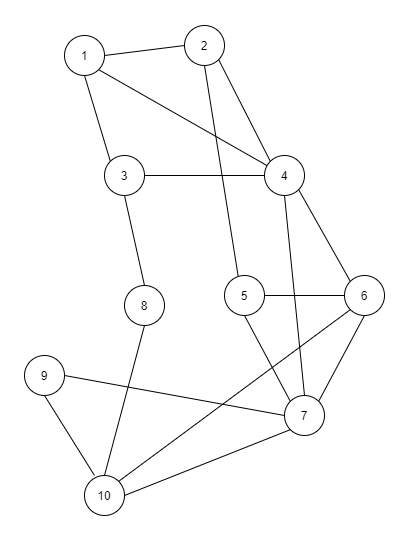
\includegraphics[scale=1.0]{g_orig}}
	\caption{Граф $G$}
	\label{fig:graph_orig}
\end{figure}

В качестве примера мы попытаемся разбить его на множества. Разобъем его на два непересекающихся множества вершин. Если мы попытаемся использовать алгоритм поиска в глубину для каждого из них, то в итоге получатся конфликтующие пути, как показано ниже на изображении \ref{fig:graph_1}.

\begin{figure}[H]
	\center{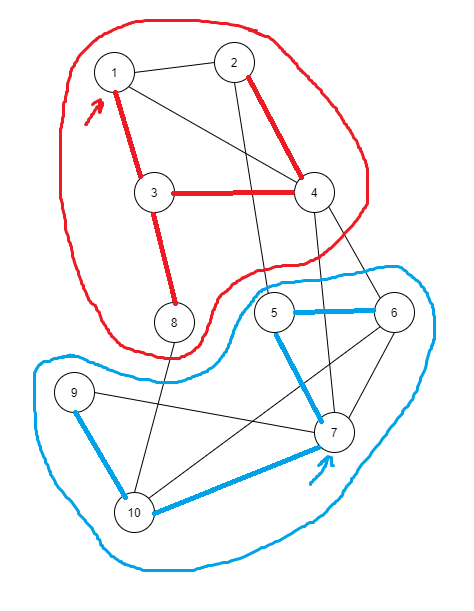
\includegraphics[scale=1.0]{g_1}}
	\caption{Граф $G$, разбитый на два пересекающихся множества}
	\label{fig:graph_1}
\end{figure}

В данном случае поиск в множестве, содержащем вершины 1, 2, 3, 4 и 8 вёлся начиная с вершины 1, во втором множестве начиная с вершины 7. В результате возникает вопрос, как корректно соединить эти множества? Возможным решением может быть использование частично пересекающихся множеств, которые имеют выраженное начало и конец, и конец предыдущего множества является начало следующего. Данная ситуация рассмотрена ниже  на рисунке \ref{fig:graph_2}.

\begin{figure}[H]
	\center{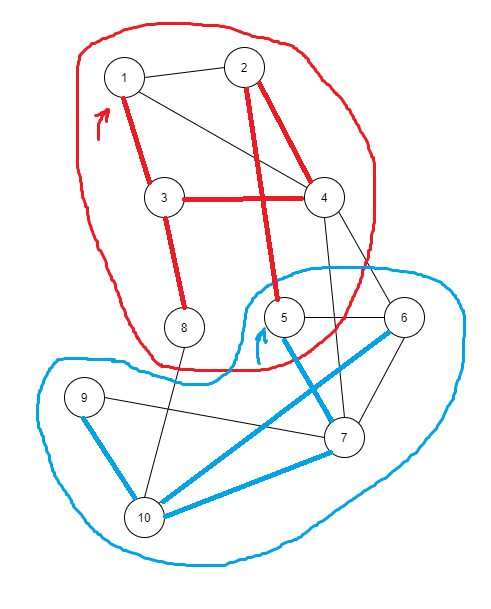
\includegraphics[scale=1.0]{g_2}}
	\caption{Граф $G$, разбитый на два частично пересекающихся множества}
	\label{fig:graph_2}
\end{figure}

В этом случае получившиеся пути не являются корректным результатом поиска в глубину, поскольку в этом случае вершина 8 была бы соединена с вершиной 10, так как дополнительные пути добавляются с конца. Для сравнения ниже на изображении  \ref{fig:g_simple} приводится результат, полученный путем применения стандартного алгоритма поиска в глубину. Стрелками помечен порядок обхода графа.

\begin{figure}[H]
	\center{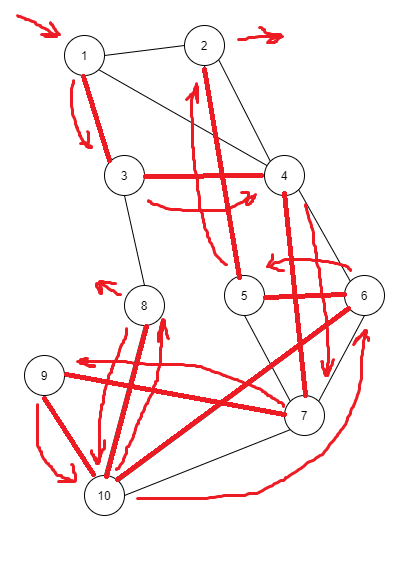
\includegraphics[scale=1.0]{g_simple}}
	\caption{Граф $G$ с результатом поиска в глубину}
	\label{fig:g_simple}
\end{figure}

Не смотря на то, что получаемые с помощью способа разбиения графа на подмножества пути могут быть достаточно близки к пути, получаемому при обходе в глубину, смысла рассматривать этот способ дальше не имеет, поскольку время, потраченное на составление и проверку пути из подмножеств полностью сведет на нет полученную в результате разбиения разницу в скорости выполнения со стандартным алгоритмом.\\

Если подробно рассмотреть работу непараллельного алгоритма поиска в глубину, то можно заметить, что множество времени тратится на обратный проход, когда необходимо найти непосещённые вершины и построить путь до них. Этот этап можно параметризировать, выполнив проверку параллельно и использовав результаты после этого.\\

\section{Анализ входных и выходных данных}
В качестве входных данных программа принимает непустой связный граф, и вершину, с которой следует начать поиск пути в глубину. На выходе программа возвращает множество найденных путей.\\

В случае параллельной реализации алгоритма к входным данным необходимо добавить количество используемых потоков.\\

\section{Анализ ограничений, в рамках которых разрабатываются алгоритмы}
На вход программе подаётся непустой связный граф, имеющий минимум одну вершину. Верхняя граница количества вершин ограничивается возможностями устройства, на котором выполняется программа.

\section{Вывод}
В данном разделе были рассмотрены основные теоретические сведения об алгоритмах поиска в глубину в графе и параллельного поиска в глубину в графе. На вход разрабатываемому алгоритму поиска в глубину на вход подаётся непустой связный граф и вершина, с которой начинается поиск. На вход разрабатываемому алгоритму параллельного поиска в глубину на вход подаётся непустой связный граф, вершина, с которой начинается поиск и количество потоков. Граф, подающийся на вход должен иметь минимум одну вершину, верхняя граница количества вершин ограничивается возможностями устройства, на котором выполняется программа. 

\chapter{Конструкторский раздел}

В данном разделе будут рассмотрены схемы, структуры данных, способы тестирования для следующих алгоритмов:
\begin{itemize}
	\item алгоритм поиска в глубину;
	\item параллельный алгоритм поиска в глубину.
\end{itemize}

\section{Алгоритм поиска в глубину}

Используемые типы и структуры данных включают в себя:
\begin{enumerate}
	\item целое число - используется для хранения и работы с целочисленными переменными;
	\item список - двунаправленный список для работы с массивами данных;
	\item узел (Node) - пользовательский класс, включающий в себя поля id (идентификатор узла) и connections (список узлов, связанных с этим узлом ребрами) и метод print\_node, выводящий информацию об узле;\\
	\item граф (Graph) - пользовательский класс, включающий в себя поле nodes (список узлов, которые составляют граф) и методы draw\_graph (вывести визуальную интерпретацию графа на экран), print\_graph (вывести все узлы), get\_node\_with\_id (возвращает объект класса Node по id).\\
\end{enumerate}

Схема алгоритма приведена на рисунках \ref{fig:algos_simple}, \ref{fig:algos_simple_rec} ниже.

\begin{figure}[H]
	\center{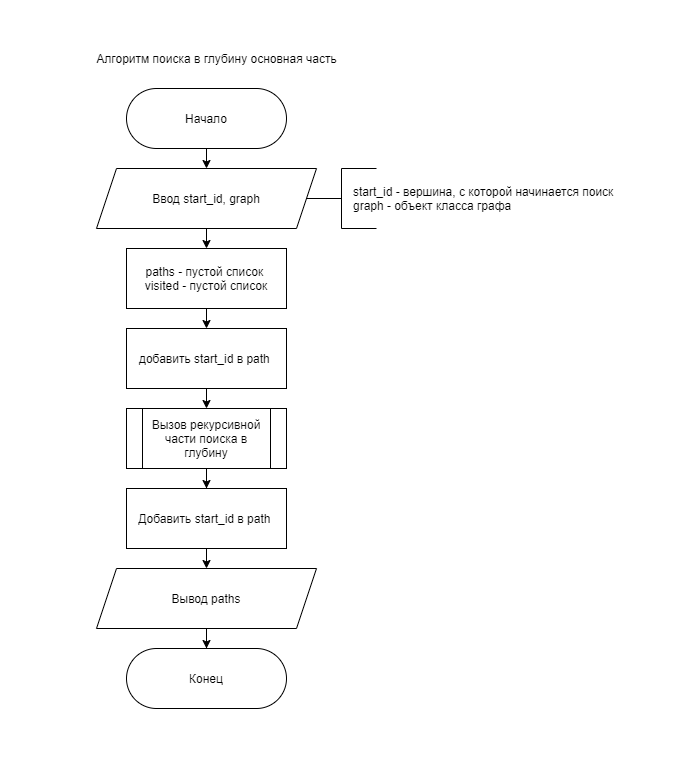
\includegraphics[scale=1.0]{algos_simple}}
	\caption{Основная часть алгоритма}
	\label{fig:algos_simple}
\end{figure}

\begin{figure}[H]
	\center{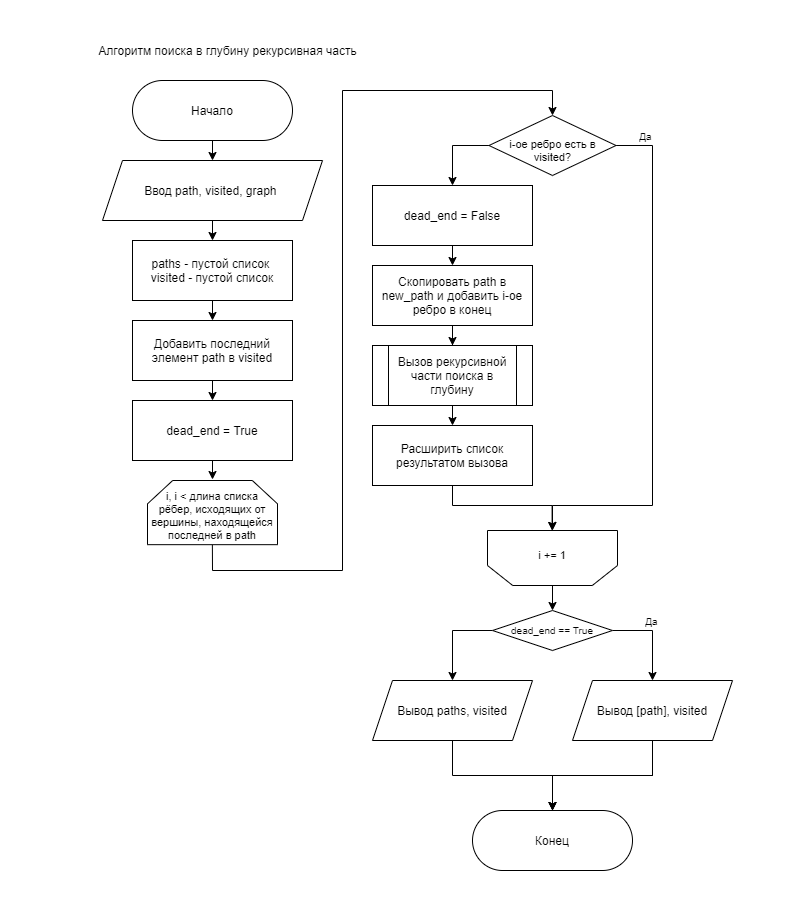
\includegraphics[scale=1.0]{algos_simple_rec}}
	\caption{Рекурсивная часть алгоритма}
	\label{fig:algos_simple_rec}
\end{figure}

\section{Алгоритм параллельного поиска в глубину}
\begin{enumerate}
	\item целое число - используется для хранения и работы с целочисленными переменными;
	\item список - двунаправленный список для работы с массивами данных;
	\item поток (Thread) - объект класса потока, позволяющий запустить выполнение функции в отдельном потоке;
	\item узел (Node) - пользовательский класс, включающий в себя поля id (идентификатор узла) и connections (список узлов, связанных с этим узлом ребрами) и метод print\_node, выводящий информацию об узле;\\
	\item граф (Graph) - пользовательский класс, включающий в себя поле nodes (список узлов, которые составляют граф) и методы draw\_graph (вывести визуальную интерпретацию графа на экран), print\_graph (вывести все узлы), get\_node\_with\_id (возвращает объект класса Node по id).\\
\end{enumerate}

Схема алгоритма приведена на рисунках \ref{fig:algos_parallel_1} - \ref{fig:algos_parallel_4} ниже.

\begin{figure}[H]
	\center{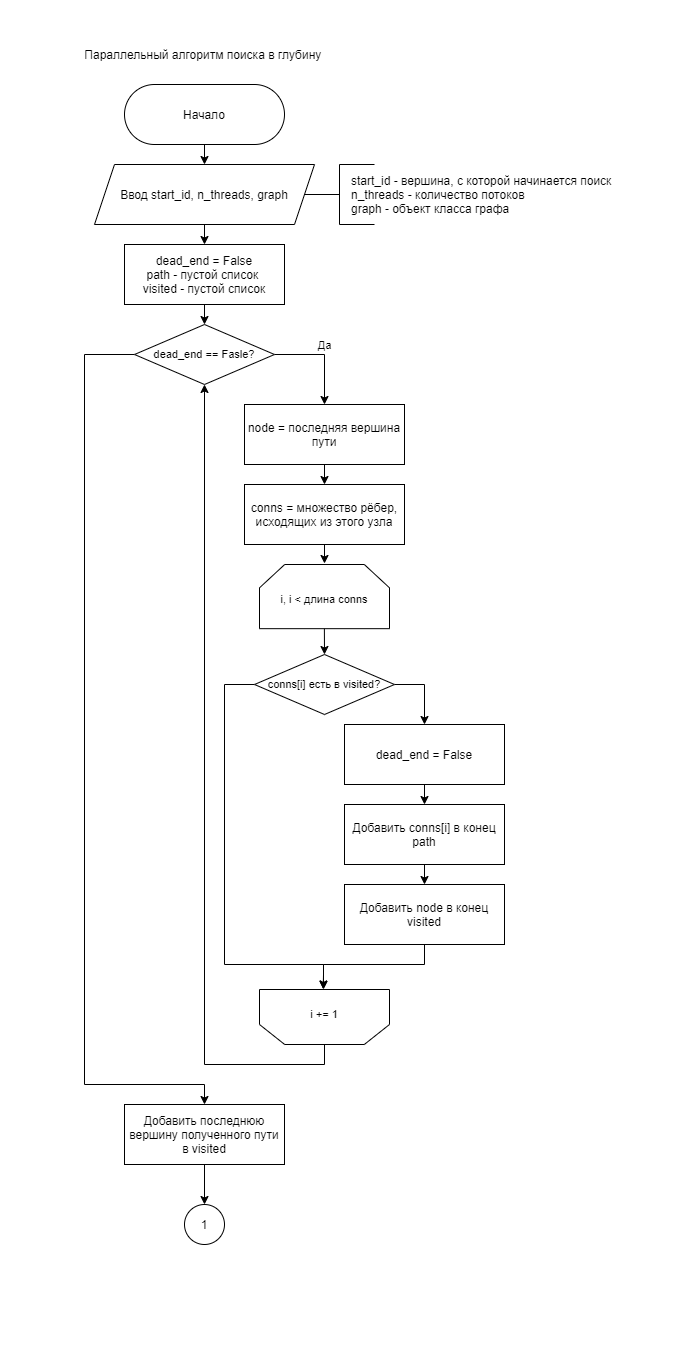
\includegraphics[scale=0.8]{algos_parallel_1}}
	\caption{Схема параллельного алгоритма, часть 1}
	\label{fig:algos_parallel_1}
\end{figure}

\begin{figure}[H]
	\center{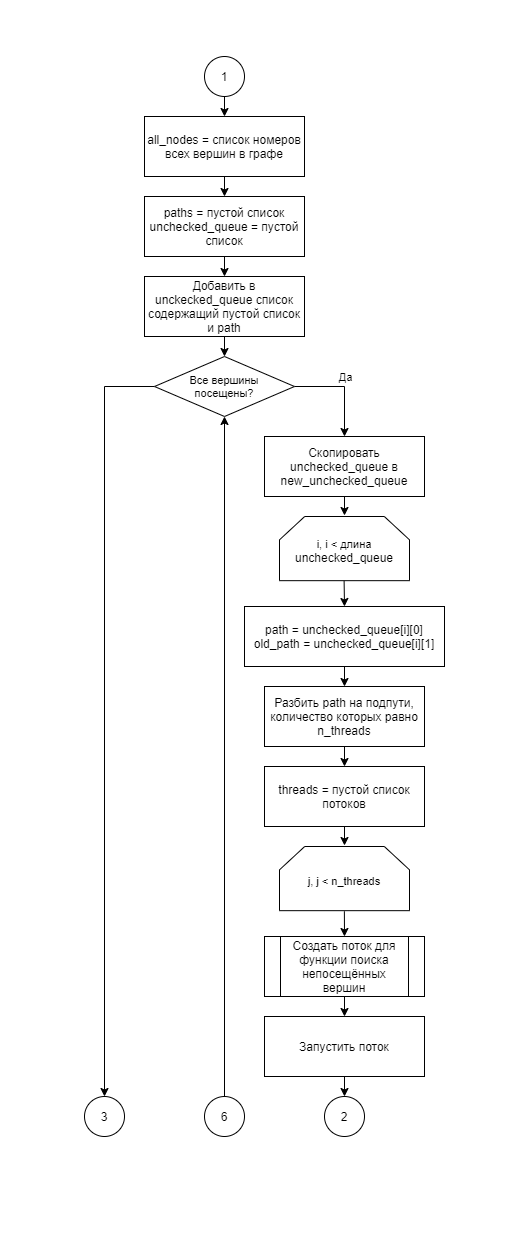
\includegraphics[scale=0.8]{algos_parallel_2}}
	\caption{Схема параллельного алгоритма, часть 2}
	\label{fig:algos_parallel_2}
\end{figure}

\begin{figure}[H]
	\center{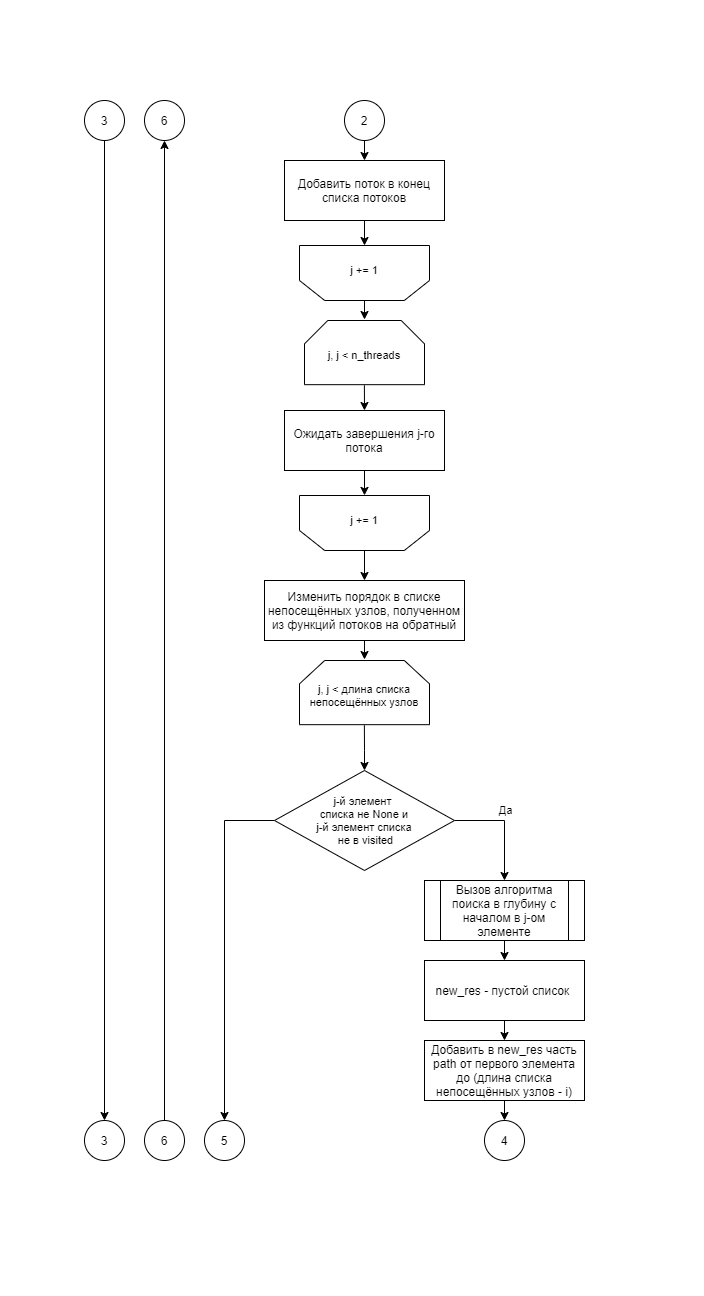
\includegraphics[scale=0.8]{algos_parallel_3}}
	\caption{Схема параллельного алгоритма, часть 3}
	\label{fig:algos_parallel_3}
\end{figure}

\begin{figure}[H]
	\center{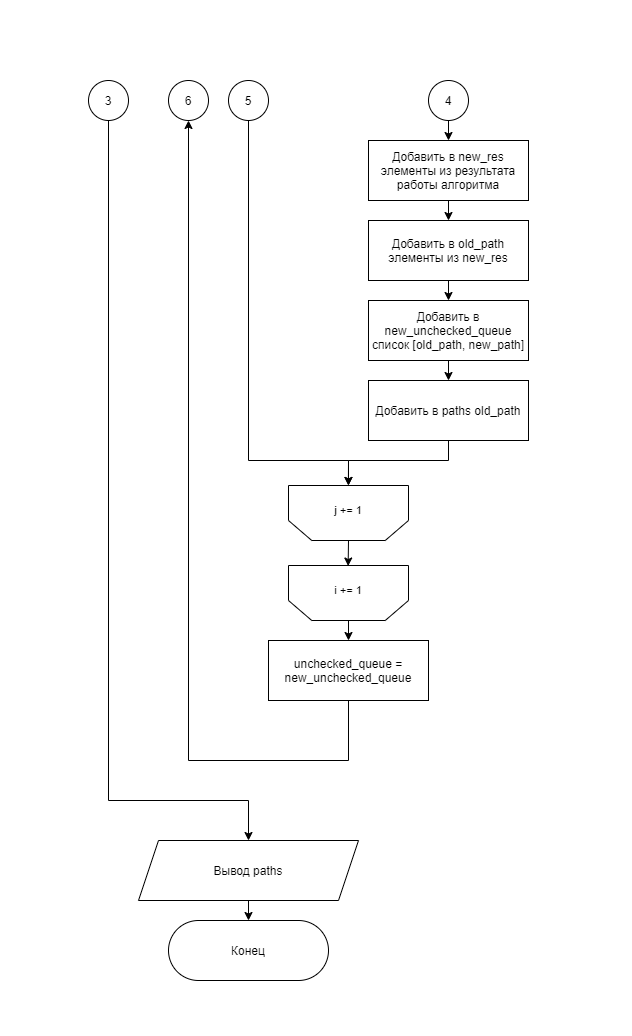
\includegraphics[scale=0.8]{algos_parallel_4}}
	\caption{Схема параллельного алгоритма, часть 4}
	\label{fig:algos_parallel_4}
\end{figure}

\section{Тестирование алгоритма поиска в глубину}

Описание тестов для алгоритам поиска в глубину:
\begin{enumerate}
	\item проверка работы на графе из одной вершины;
	\item проверка работы на графе из чётного количества вершин;
	\item проверка работы на графе из нечётного количества вершин;
\end{enumerate}

\section{Функциональная схема ПО}
На изображении ниже представлена функиональная схема разрабатываемого ПО. На вход подаётся граф, идентификатор вершины, с которой начинается поиск и количество потоков, при помощи алгоритмов, реализованных на языке Python мы получаем в результате работы множество найденных путей.

\begin{figure}[ph!]
	\center{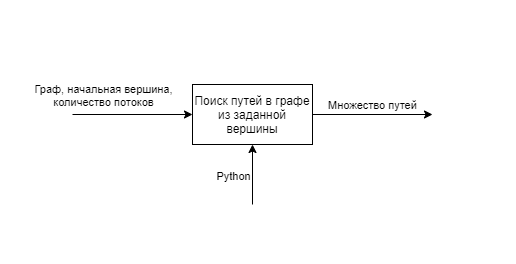
\includegraphics[scale=1.0]{func_scheme}}
	\caption{IDEF0 диаграмма разрабатываемой программы}
\end{figure}

\section{Вывод}
В данном разделе были рассмотрены схемы алгоритма поиска в глубину, параллельного алгоритма поиска в глубину. Были определены тесты для каждого алгоритма и описаны типы и структуры данных, использующихся в алгоритмах. Также была приведена функциональная схема разрабатываемого ПО.

\chapter{Технологический раздел}

В данном разделе будут рассмотрены подробности реализации описаных выше алгоритмов. Также будут обоснованы выбор языка программирования для реализации, выбор библиотек для проведения экспериментов и представлены важные фрагменты кода написанной в рамках работы программы.

\section{Выбор языка программирования}

В качестве языка программирования для реализации данной лабораторной работы использовался язык программирования Python поскольку он предоставляет широкие возможности для эффективной реализации алгоритмов. В качестве среды разработки использовалась Visual Studio Code по причине того, что данная среда имеет встроенные средства отладки и анализа работы программы, позволяющие быстро и эффективно писать код.

\section{Сведения о модулях программы}

Реализованное ПО состоит из трёх модулей:
\begin{enumerate}
	\item main - основной файл программы, где находится точка входа;
	\item simple\_dfs - реализация рекурсивного алгоритма поиска в глубину;
	\item paralle\_dfs - реализация параллельного алгоритма поиска в глубину;
	\item test - реализация тестирования;
	\item time - реализация тестирования временной производительности;
	\item graph - реализация классов графа и вершины.
\end{enumerate}

\section{Реализация алгоритмов}

\begin{lstlisting}[label=some-code-1,caption=Реализация алгоритма поиска в глубину]
def simple_dfs(self, start_id: int, graph: Graph) -> list[list[int]]:
    path = [start_id]
    visited = []
    paths, _ = self.simple_dfs_rec(path, visited, graph)
    return paths

def simple_dfs_rec(self, path: list[int], visited: list[int], graph: Graph) -> list[list[int]]:
    paths = []
    visited.append(path[-1])
    dead_end = True
    for conn in graph.get_node_with_id(path[-1]).connections:
        if conn not in visited:
            dead_end = False
            new_path = path.copy()
            new_path.append(conn)
            res_path, visited = self.simple_dfs_rec(new_path, visited, graph)
            paths.extend(res_path)
            
    if dead_end:
        return [path], visited
    else:
        return paths, visited
\end{lstlisting}

\begin{lstlisting}[label=some-code-2,caption=Реализация параллельного алгоритма поиска в глубину]

def parallel_search_unvisited(self, node_ids: list[int], return_ids: list[list[int]], index: int, visited: set[int], graph: Graph):
    return_id = [None] * len(node_ids)

    for i in range(0, len(node_ids)):
        conns = graph.get_node_with_id(node_ids[i]).connections
        for j in range(0, len(conns)):
            if conns[j] not in visited:
                return_id[i] = conns[j]
                break
    return_ids[index] = return_id

def parallel_dfs_subgraph(self, start_id: int, visited: set[int], graph: Graph):
    dead_end = False
    path = [start_id]
    visited.add(start_id)
    node = path[-1]

    while not dead_end:
        conns = graph.get_node_with_id(node).connections
        dead_end = True
        for conn in conns:
            if conn not in visited:
                dead_end = False
                path.append(conn)
                node = conn
                visited.add(conn)
                break

    return path, visited
    

def parallel_dfs(self, start_id: int, n_threads: int, graph: Graph):
    dead_end = False
    path = [start_id]
    visited = set()

    while not dead_end:
        node = path[-1]
        conns = graph.get_node_with_id(node).connections
        
        dead_end = True
        for conn in conns:
            if conn not in visited and dead_end:
                dead_end = False
                path.append(conn)
                visited.add(node)
    
    visited.add(path[-1])

    all_nodes = set()
    for node in graph.nodes:
        all_nodes.add(node.id)
    
    paths = [path]        
    unchecked_queue = [[[], path]]

    while len(all_nodes) != len(visited):
        new_unchecked_queue = unchecked_queue.copy()
        for pair in unchecked_queue:
            path = pair[1]
            old_path = pair[0]

            # find unchecked nodes
            node_index = 0
            batch_size = ceil(len(path) / n_threads)
            batches = []
            batch = []

            path_len = len(path)
            while node_index < path_len:
                batch.append(path[node_index])
                if len(batch) == batch_size:
                    batches.append(batch)
                    batch = []
                node_index += 1

            if len(batch) > 0:
                if len(batches) == 0:
                    batches.append(batch)
                else:
                    batches[-1].extend(batch)

            sum_size = 0
            for batch in batches:
                sum_size += len(batch)

            result_ids = [[]] * len(batches)
            index = 0
            threads = []

            for batch in batches:
                thread = Thread(target=self.parallel_search_unvisited, args=(batch, result_ids, index, visited, graph))
                thread.start()
                threads.append(thread)
                index += 1

            for thread in threads:
                thread.join()
            
            result_pass = []
            for result_id in result_ids:
                result_pass.extend(result_id)
            result_pass.reverse() # this list contains inverted next node to check in path

            # search for unvisited vertex
            res_pass_len = len(result_pass)
            for i in range(0, res_pass_len):
                if result_pass[i] != None and result_pass[i] not in visited:
                    new_path, visited = self.parallel_dfs_subgraph(result_pass[i], visited, graph)
                    new_res = path[:(res_pass_len - i)]
                    new_res.extend(new_path)
                    old_path.extend(new_res)
                    new_unchecked_queue.append([old_path, new_path]) # adding path and last added node to unchecked queue
                    paths.append(old_path)
        unchecked_queue = new_unchecked_queue

    return paths
\end{lstlisting}

\section{Результаты тестирования алгоритмов}

Для тестирования алгоритмов было реализованы следующие тесты:
\begin{enumerate}
	\item проверка работы на графе из одного элемента;
	\item проверка работы на ключе из середины словаря;
\end{enumerate}

Результаты тестов:

\section{Вывод}
В данной разделе были представлены реализации алгоритма полного перебора, бинарного поиска и частичного анализа, а также представлены результаты работы модуля тестирования реализованных алгоритмов.

\chapter{Экспериментальный раздел}

В данном разделе описываются измерения временных характеристики алгоритмов полного перебра, бинарного поиска и частичного анализа для различных положений ключа в словаре, а также делается вывод об эффективности алгоритмов для соответствующих случаев.

\section{Технические характеристики}
\begin{itemize}
	\item Операционная система - Windows 10, 64-bit;
	\item Оперативная память - 16 GiB;
	\item Процессор - Intel(R) Core(TM) i7-9750H CPU @ 2.60GHz 2.59 GHz, 6 ядер, 12 потоков.
\end{itemize}

\section{Результаты экспериментов}
В данном разделе рассматриваются результаты экспериментов над разработанными алгоритмами. Результаты приведены ниже в таблицах \ref{tab:thr_1} -  \ref{tab:thr_8} и на графиках \ref{fig:res_thr_1} - \ref{fig:res_thr_8}.

\begin{table}[H]
  \begin{center}
    \captionsetup{justification=raggedright}
     \caption{Время работы алгоритмов для одного потока}
    \label{tab:thr_1}
    \begin{tabular}{|c|c|c|}
      \hline	
      \textbf{количество узлов} & \textbf{t не параллельного (нс)}  & \textbf{t не параллельного (нс)}\\
      \hline	
	100 & 1562500.0 & 1562500.0\\
	150 & 6250000.0 & 9375000.0\\     
	200 & 4687500.0 & 10937500.0\\    
	250 & 1562500.0 & 20312500.0\\    
	300 & 10937500.0 & 21875000.0\\   
	350 & 12500000.0 & 25000000.0\\   
	400 & 15625000.0 & 29687500.0\\   
	450 & 18750000.0 & 37500000.0\\   
	500 & 28125000.0 & 40625000.0\\   
	550 & 34375000.0 & 40625000.0\\   
	600 & 37500000.0 & 42187500.0\\   
	650 & 43750000.0 & 62500000.0\\   
	700 & 48437500.0 & 42187500.0\\   
	750 & 59375000.0 & 59375000.0\\   
	800 & 70312500.0 & 56250000.0\\   
	850 & 78125000.0 & 84375000.0\\   
	900 & 84375000.0 & 98437500.0\\   
	950 & 103125000.0 & 125000000.0\\ 
	1000 & 123437500.0 & 107812500.0\\
	1050 & 134375000.0 & 117187500.0\\
	1100 & 148437500.0 & 143750000.0\\
	1150 & 153125000.0 & 132812500.0\\
	1200 & 165625000.0 & 162500000.0\\
	1250 & 196875000.0 & 162500000.0\\
	1300 & 192187500.0 & 195312500.0\\
	1350 & 207812500.0 & 198437500.0\\
	1400 & 218750000.0 & 268750000.0\\
	1450 & 229687500.0 & 276562500.0\\
	1500 & 273437500.0 & 234375000.0\\
      \hline	
    \end{tabular}
  \end{center}
\end{table}

\begin{figure}[H]
	\center{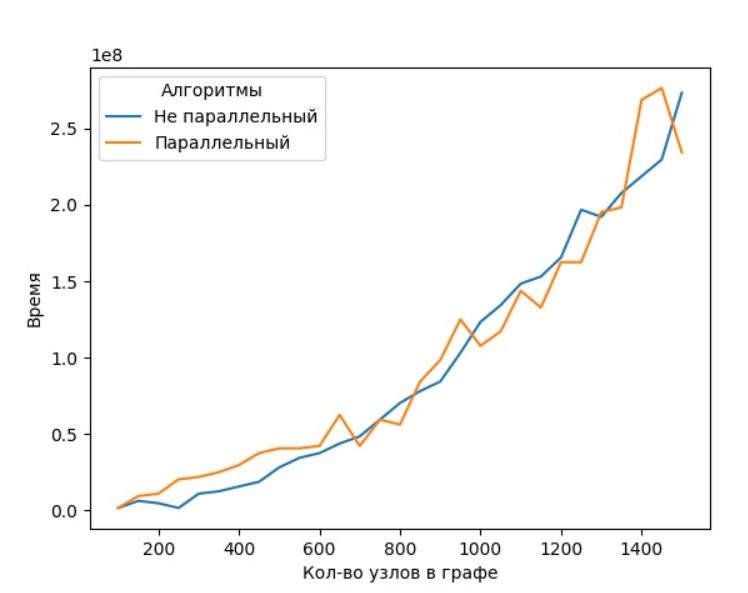
\includegraphics[scale=0.8]{res_thr_1}}
	\caption{График зависимости времени работы параллельного и непараллельного алгоритмов в зависимости от количества узлов для одного потока}
	\label{fig:res_thr_1}
\end{figure}

\begin{table}[H]
  \begin{center}
    \captionsetup{justification=raggedright}
     \caption{Время работы алгоритмов для двух потоков}
    \label{tab:thr_2}
    \begin{tabular}{c|c|c}
      \textbf{количество узлов} & \textbf{время не параллельного (нс)}  & \textbf{время не параллельного (нс)}\\
	100 & 1562500.0 & 6250000.0\\
	150 & 4687500.0 & 10937500.0\\
	200 & 4687500.0 & 7812500.0\\
	250 & 4687500.0 & 14062500.0\\
	300 & 7812500.0 & 12500000.0\\
	350 & 15625000.0 & 18750000.0\\
	400 & 15625000.0 & 29687500.0\\
	450 & 20312500.0 & 26562500.0\\
	500 & 25000000.0 & 34375000.0\\
	550 & 31250000.0 & 40625000.0\\
	600 & 32812500.0 & 34375000.0\\
	650 & 45312500.0 & 45312500.0\\
	700 & 57812500.0 & 51562500.0\\
	750 & 59375000.0 & 56250000.0\\
	800 & 71875000.0 & 60937500.0\\
	850 & 79687500.0 & 78125000.0\\
	900 & 84375000.0 & 79687500.0\\
	950 & 93750000.0 & 81250000.0\\
	1000 & 101562500.0 & 89062500.0\\
	1050 & 115625000.0 & 90625000.0\\
	1100 & 126562500.0 & 146875000.0\\
	1150 & 145312500.0 & 128125000.0\\
	1200 & 154687500.0 & 126562500.0\\
	1250 & 173437500.0 & 154687500.0\\
	1300 & 178125000.0 & 139062500.0\\
	1350 & 200000000.0 & 164062500.0\\
	1400 & 209375000.0 & 206250000.0\\
	1450 & 223437500.0 & 242187500.0\\
	1500 & 239062500.0 & 231250000.0\\
      \hline	
    \end{tabular}
  \end{center}
\end{table}

\begin{figure}[H]
	\center{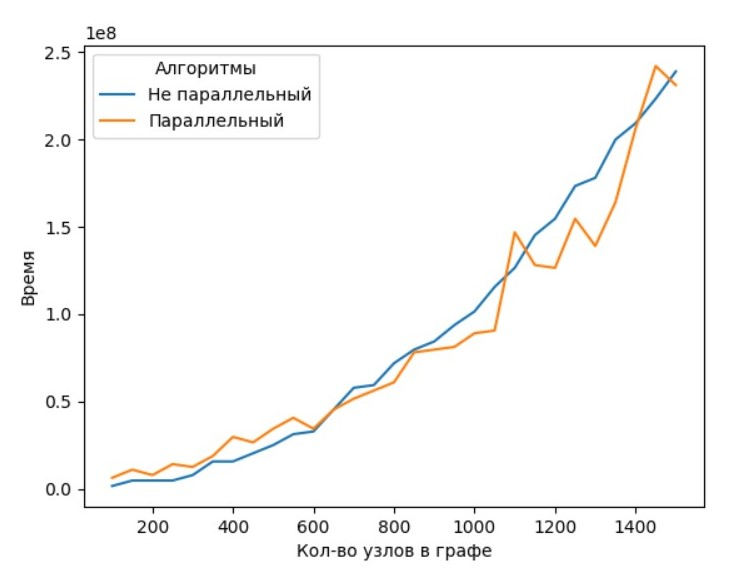
\includegraphics[scale=0.8]{res_thr_2}}
	\caption{График зависимости времени работы параллельного и непараллельного алгоритмов в зависимости от количества узлов для двух потоков}
	\label{fig:res_thr_2}
\end{figure}

\begin{table}[H]
  \begin{center}
    \captionsetup{justification=raggedright}
     \caption{Время работы алгоритмов для четырех потоков}
    \label{tab:thr_4}
    \begin{tabular}{c|c|c}
      \textbf{количество узлов} & \textbf{время не параллельного (нс)}  & \textbf{время не параллельного (нс)}\\
	100 & 0.0 & 1562500.0\\
	150 & 4687500.0 & 3125000.0\\
	200 & 4687500.0 & 7812500.0\\
	250 & 7812500.0 & 9375000.0\\
	300 & 10937500.0 & 14062500.0\\
	350 & 15625000.0 & 14062500.0\\
	400 & 17187500.0 & 25000000.0\\
	450 & 25000000.0 & 18750000.0\\
	500 & 29687500.0 & 26562500.0\\
	550 & 34375000.0 & 32812500.0\\
	600 & 39062500.0 & 35937500.0\\
	650 & 46875000.0 & 46875000.0\\
	700 & 54687500.0 & 50000000.0\\
	750 & 68750000.0 & 56250000.0\\
	800 & 85937500.0 & 64062500.0\\
	850 & 85937500.0 & 64062500.0\\
	900 & 93750000.0 & 78125000.0\\
	950 & 104687500.0 & 79687500.0\\
	1000 & 117187500.0 & 89062500.0\\
	1050 & 135937500.0 & 98437500.0\\
	1100 & 148437500.0 & 139062500.0\\
	1150 & 162500000.0 & 117187500.0\\
	1200 & 170312500.0 & 137500000.0\\
	1250 & 181250000.0 & 140625000.0\\
	1300 & 193750000.0 & 157812500.0\\
	1350 & 206250000.0 & 145312500.0\\
	1400 & 206250000.0 & 176562500.0\\
	1450 & 229687500.0 & 160937500.0\\
	1500 & 243750000.0 & 200000000.0\\
      \hline	
    \end{tabular}
  \end{center}
\end{table}

\begin{figure}[H]
	\center{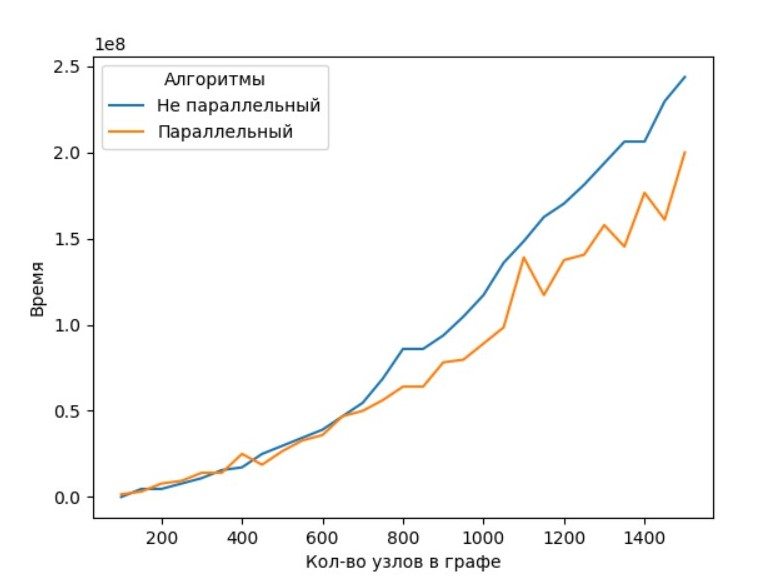
\includegraphics[scale=0.8]{res_thr_4}}
	\caption{График зависимости времени работы параллельного и непараллельного алгоритмов в зависимости от количества узлов для четырёх потоков}
	\label{fig:res_thr_4}
\end{figure}

\begin{table}[H]
  \begin{center}
    \captionsetup{justification=raggedright}
     \caption{Время работы алгоритмов для восьми потока}
    \label{tab:thr_8}
    \begin{tabular}{c|c|c}
      \textbf{количество узлов} & \textbf{время не параллельного (нс)}  & \textbf{время не параллельного (нс)}\\
	100 & 0.0 & 1562500.0\\
	150 & 3125000.0 & 3125000.0\\     
	200 & 14062500.0 & 1562500.0\\    
	250 & 6250000.0 & 9375000.0\\     
	300 & 12500000.0 & 10937500.0\\   
	350 & 14062500.0 & 14062500.0\\   
	400 & 17187500.0 & 23437500.0\\   
	450 & 26562500.0 & 20312500.0\\   
	500 & 29687500.0 & 20312500.0\\   
	550 & 34375000.0 & 25000000.0\\   
	600 & 40625000.0 & 37500000.0\\   
	650 & 46875000.0 & 40625000.0\\   
	700 & 54687500.0 & 42187500.0\\   
	750 & 67187500.0 & 48437500.0\\   
	800 & 76562500.0 & 50000000.0\\   
	850 & 90625000.0 & 67187500.0\\   
	900 & 93750000.0 & 78125000.0\\   
	950 & 123437500.0 & 75000000.0\\  
	1000 & 115625000.0 & 93750000.0\\ 
	1050 & 135937500.0 & 90625000.0\\ 
	1100 & 145312500.0 & 100000000.0\\
	1150 & 160937500.0 & 114062500.0\\
	1200 & 168750000.0 & 129687500.0\\
	1250 & 185937500.0 & 132812500.0\\
	1300 & 210937500.0 & 139062500.0\\
	1350 & 229687500.0 & 160937500.0\\
	1400 & 239062500.0 & 151562500.0\\
	1450 & 259375000.0 & 190625000.0\\
	1500 & 275000000.0 & 179687500.0\\
      \hline	
    \end{tabular}
  \end{center}
\end{table}

\begin{figure}[H]
	\center{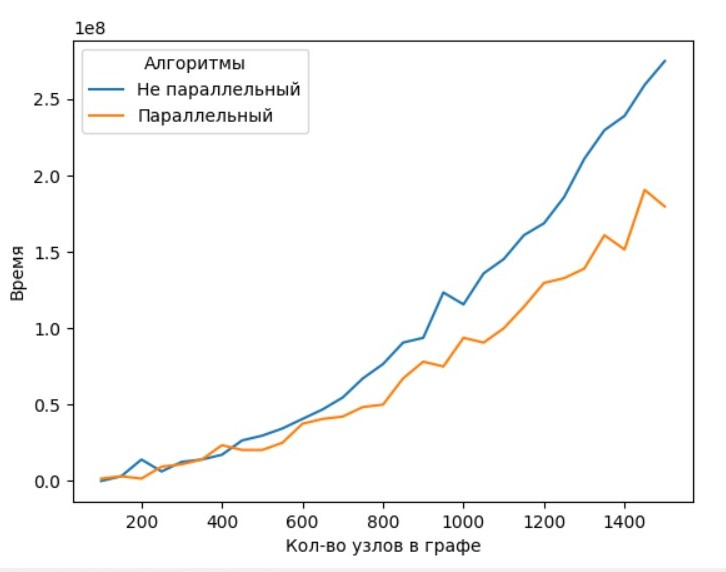
\includegraphics[scale=0.8]{res_thr_8}}
	\caption{График зависимости времени работы параллельного и непараллельного алгоритмов в зависимости от количества узлов для пяти потоков}
	\label{fig:res_thr_8}
\end{figure}

\section{Вывод}
В результате экспериментов было получено, что при использовании параллельного метода при небольших размерах графа разница не является значительной, однако при использовании 8 потоков при размере 1500 узлов достигается ускорение в 1.5 раза.